% A LaTeX template fitted for a Phd thesis report
% Copyright (C) 2013 Damien Roque

% This program is free software; you can redistribute it and/or
% modify it under the terms of the GNU General Public License
% as published by the Free Software Foundation; either version 2
% of the License, or (at your option) any later version.

% This program is distributed in the hope that it will be useful,
% but WITHOUT ANY WARRANTY; without even the implied warranty of
% MERCHANTABILITY or FITNESS FOR A PARTICULAR PURPOSE.  See the
% GNU General Public License for more details.

% You should have received a copy of the GNU General Public License
% along with this program; if not, write to the Free Software
% Foundation, Inc., 51 Franklin Street, Fifth Floor, Boston, MA  02110-1301, USA.

% Author : Damien Roque <damien.roque@gipsa-lab.grenoble-inp.fr>

\documentclass[a4paper,11pt,twoside]{templates/roque-phdthesis-template}

% Include configuration (loading packages, defining the style of the document...)
\usepackage[utf8]{inputenc}
\RequirePackage[l2tabu, orthodox]{nag} % check all packages

\usepackage[a4paper]{templates/first-page-udg}

% Encoding and internationalization
\usepackage[T1]{fontenc}
\usepackage{aecompl}
\usepackage[utf8]{inputenc}  % For accent
% \usepackage[french]{babel} % Comment this line if the document is written in english
\usepackage[american]{babel} % Comment this line if the document is written in english

% Math packages
\usepackage{amsmath,amssymb}
\usepackage{mathrsfs}
\usepackage{amsthm}
\usepackage{a4wide}
\renewcommand{\baselinestretch}{1.05}

% Mini table of content and acronyms
\usepackage[nottoc, notlof, notlot]{tocbibind}
\usepackage[french]{minitoc}
\setcounter{minitocdepth}{2}
\mtcindent=15pt
\setlength{\parskip}{10pt}

\let\minitocORIG\minitoc
\renewcommand{\minitoc}{\minitocORIG \vspace{1.5em}}

\setcounter{secnumdepth}{3}
\setcounter{tocdepth}{2}

% Graphics and hyperlinks
\usepackage{ifpdf}
\ifpdf
  \usepackage[pdftex]{graphicx}
  \DeclareGraphicsExtensions{.jpg,.pdf,.png}
  %\usepackage[a4paper,pagebackref,hyperindex=true]{hyperref}
  \usepackage[a4paper,hyperindex=true]{hyperref}
\else
  \usepackage{graphicx}
  \DeclareGraphicsExtensions{.ps,.eps}
  %\usepackage[a4paper,dvipdfm,pagebackref,hyperindex=true]{hyperref}
  \usepackage[a4paper,dvipdfm,hyperindex=true]{hyperref}
\fi
\graphicspath{{.}{images/}}
\usepackage{eso-pic}
\usepackage{rotating}
\usepackage[font=normalsize]{subfig}
\usepackage{tikz}
\usetikzlibrary{shapes,arrows}
\usepackage{pgfplots}
\pgfplotsset{compat=newest}
\pgfplotsset{plot coordinates/math parser=false}
\newlength\figureheight
\newlength\figurewidth

\pgfkeys{/pgf/number format/.cd,
set decimal separator={,\!},
1000 sep={\,},
} % Comment this line if the document is written in english

\usetikzlibrary{plotmarks}
\usepackage{pdfpages}

\usepackage[strict]{changepage}
\newcommand\BackgroundPic{
\put(0,0){
\parbox[b][\paperheight]{\paperwidth}{%
\vfill
\centering

\includegraphics[width=0.9\paperwidth,height=1\paperheight,keepaspectratio]{images/background-eps-converted-to}%
\vfill
}}}

\usepackage{color}
\definecolor{linkcol}{rgb}{0,0,0} 
\definecolor{citecol}{rgb}{0,0,0}

\hypersetup
{
bookmarksopen=true,
pdftitle={Mon sujet de thèse complet},
pdfauthor={Prénom NOM},
pdfsubject={Rapport de thèse},
pdfmenubar=true,
pdfhighlight=/O,
colorlinks=true,
pdfpagemode=None,
pdfpagelayout=SinglePage,
pdffitwindow=true,
linkcolor=linkcol,
citecolor=citecol,
urlcolor=linkcol
}



% Headers and footers
\usepackage{fancyhdr}
\pagestyle{fancy}
\fancyfoot{}
\fancyhead[LE,RO]{\bfseries\thepage}
\fancyhead[RE]{\bfseries\nouppercase{\leftmark}}
\fancyhead[LO]{\bfseries\nouppercase{\rightmark}}

\let\headruleORIG\headrule
\renewcommand{\headrule}{\color{black} \headruleORIG}
\renewcommand{\headrulewidth}{1.0pt}
\usepackage{colortbl}
\arrayrulecolor{black}

\fancypagestyle{plain}{
  \fancyhead{}
  \fancyfoot[C]{\thepage}
  \renewcommand{\headrulewidth}{0pt}
}

\usepackage[footnote]{acronym}

% References formatting
% Bibtex
% \renewcommand*{\backref}[1]{}
% \renewcommand*{\backrefalt}[4]{%
% \ifcase #1 %
% (Non cité.)%
% \or
% (Cité en page~#2.)%
% \else
% (Cité en pages~#2.)%
% \fi}
% \renewcommand*{\backrefsep}{, }
% \renewcommand*{\backreftwosep}{ et~}
% \renewcommand*{\backreflastsep}{ et~}

% BibLatex
\usepackage[style=alphabetic-verb,backend=bibtex,isbn=false,doi=false,backref=true,url=false]{biblatex}
\addbibresource{references.bib}

% Pages succession
\makeatletter
\def\cleardoublepage{\clearpage\if@twoside \ifodd\c@page\else%
  \hbox{}%
  \thispagestyle{empty}%
  \newpage%
  \if@twocolumn\hbox{}\newpage\fi\fi\fi}
\makeatother

\newenvironment{vcenterpage}
{\newpage\vspace*{\fill}\thispagestyle{empty}\renewcommand{\headrulewidth}{0pt}}
{\vspace*{\fill}}

%%% Local Variables: 
%%% mode: latex
%%% TeX-master: "../roque-phdthesis"
%%% End: 


%% TO DO
\usepackage{titlesec}
\titleclass{\part}{top}
\titleformat{\part}[display]
{\normalfont\huge\bfseries}{\centering\partname\ \thepart}{20pt}{\Huge\centering}
\titlespacing*{\part}{0pt}{50pt}{40pt}
%\titleclass{\chapter}{straight}
%\titleformat{\chapter}[display]
%{\normalfont\huge\bfseries}{\chaptertitlename\ \thechapter}{20pt}{\Huge}
%\titlespacing*{\chapter} {0pt}{50pt}{40pt}


\usepackage{amsmath,amsfonts}

% Top 9 packages
% \usepackage{microtype}
% The microtype package improves the spacing between words and letters. It does a lot more and most people won’t notice the difference. But still, the resulting document will be easier to read and looks better when microtype is loaded. Load this package after fonts, if any, as the package behavior is dependent on this font. - See more at: http://www.howtotex.com/packages/9-essential-latex-packages-everyone-should-use/#sthash.e5Qsr4ay.dpuf
% \usepackage{siunitx}
% The siunitx package greatly simplifies TeXing when writing scientific documents, where units and numbers are a big part of the writing. This package adds commands like \num for typesetting numbers in all sorts of ways and \si for units. The commands I use a lot are \SI and \SIrange. For example, \SI{10}{\hertz} results in ‘10Hz‘ in text (this is especially useful to prevent typo’s; I tend to write HZ or hz a lot instead of Hz). The \SIrange command requires one more input variable: \SIrange{10}{100}{\hertz} produces ‘10Hz to 100Hz‘. Note that the siunitx package was already featured in an earlier post on this blog. - See more at: http://www.howtotex.com/packages/9-essential-latex-packages-everyone-should-use/#sthash.e5Qsr4ay.dpuf
% \usepackage{cleveref}
% Another fascinating LaTeX package is cleveref. This package introduces the \cref command. When using this command to make cross-references, instead of \ref or \eqref, a word is placed in front of the reference according to the type of reference: fig. for figures, eq. for equations. Hence, another LaTeX package that simplifies the writing. The package was earlier mentioned in this post. In that post it is also shown how to change the words in front of references. - See more at: http://www.howtotex.com/packages/9-essential-latex-packages-everyone-should-use/#sthash.e5Qsr4ay.dpuf
% \usepackage[colorlinks=false, pdfborder={0 0 0}]{hyperref} 
% See more at: http://www.howtotex.com/packages/9-essential-latex-packages-everyone-should-use/#sthash.e5Qsr4ay.dpuf
% \usepackage{booktabs}
% The booktabs package allows you to create tables without vertical separators. These separators are just unnecessary and plain ugly. Creating a table with booktabs is however more of a pain than the normal way of creating LaTeX tables. Therefore, I dedicated a post on how to create nice tables with the booktabs package earlier. - See more at: http://www.howtotex.com/packages/9-essential-latex-packages-everyone-should-use/#sthash.e5Qsr4ay.dpuf
\usepackage{todonotes}

% Include user's macros
% Math macros
\newcommand*{\SET}[1]  {\ensuremath{\mathrm{\mathbf{#1}}}}
\newcommand*{\VEC}[1]  {\ensuremath{\boldsymbol{#1}}}
\newcommand*{\MAT}[1]  {\ensuremath{\boldsymbol{#1}}}
\newcommand*{\OP}[1]  {\ensuremath{\boldsymbol{\mathcal{#1}}}}
\newcommand*{\ESP}[1]  {\ensuremath{ \mathbb{E} \left \{#1 \right \}}}
\newcommand*{\ESPENS}[2]  {\ensuremath{ \mathbb{E}_{#1} \left \{#2 \right \}}}
\newcommand*{\NORM}[1]  {\ensuremath{\left\|#1\right\|}}
\newcommand*{\DPR}[2]  {\ensuremath{\left \langle #1,#2 \right \rangle}}
\newcommand*{\FOURIER}[1]  {\ensuremath{\widehat{#1}}}
\newcommand{\eqdef}{\stackrel{\mathrm{def}}{=}}
\newcommand{\argmax}{\operatornamewithlimits{argmax }}
\newcommand{\argmin}{\operatornamewithlimits{argmin }}
%\newcommand{\argmin}{\arg\!\min}
\newcommand{\diag}{\operatorname{diag}}
\newcommand{\ud}{\, \mathrm{d}}
\newcommand{\vect}{\mathrm{Vect}}
\newcommand{\sinc}{\mathrm{sinc}}
\newcommand{\esp}{\ensuremath{\mathrm{E}}} % Problème pour les short captions
\newcommand{\hilbert}{\ensuremath{\mathcal{H}}}
\newcommand{\supps}{\ensuremath{\tilde{\mathrm{supp}}}}
\newcommand{\supp}{\ensuremath{\mathrm{supp}}}
\newcommand{\sgn}{\mathrm{sgn}}
\newcommand{\intTT}{\int_{-T}^{T}}
\newcommand{\intT}{\int_{-\frac{T}{2}}^{\frac{T}{2}}}
\newcommand{\intinf}{\int_{-\infty}^{+\infty}}
\newcommand{\iintinf}{\iint_{-\infty}^{+\infty}}
\newcommand{\iintrr}{\iint\limits_{\SET{R}^2}}
\newcommand{\intr}{\int\limits_{\R}}
\newcommand{\Sh}{\ensuremath{\boldsymbol{U}}}
\newcommand{\C}{\ensuremath{\mathbf{C}}}
\newcommand{\R}{\ensuremath{\mathbf{R}}}
\newcommand{\Z}{\ensuremath{\mathbf{Z}}}
\newcommand{\N}{\ensuremath{\mathbf{N}}}
\newcommand{\K}{\ensuremath{\mathbf{K}}}
\newcommand{\reel}{\mathcal{R}}
\newcommand{\imag}{\mathcal{I}}
\newcommand{\cmnr}{c_{m,n}^\reel}
\newcommand{\cmni}{c_{m,n}^\imag}
\newcommand{\cnr}{c_{n}^\reel}
\newcommand{\cni}{c_{n}^\imag}
\newcommand{\tproto}{g}
\newcommand{\rproto}{\check{g}}
\newcommand{\Tproto}{G}
\newcommand{\Rproto}{\check{G}}
\newcommand{\Tpoly}{F}
\newcommand{\Rpoly}{\check{F}}
\newcommand{\estim}{\tilde{c}}
\newcommand{\egal}{\bar{c}}
\newcommand{\bb}{b}
\newcommand{\bbf}{z}
\newcommand{\bbr}{\zeta}
\newcommand{\LR}{\mathcal{L}_2(\R)}
\newcommand{\LRR}{\mathcal{L}_2(\R^2)}
\newcommand{\LZ}{\ell_2(\Z)}
\newcommand{\LZZ}{\ell_2(\Z^2)}
\newcommand{\peigne}{\ensuremath{\Psi}}
\newcommand{\avec}{\qquad \text{avec} \qquad}

% Theorems definition
\newtheoremstyle{break}
  {11pt}{11pt}%
  {\itshape}{}%
  {\bfseries}{}%
  {\newline}{}%
\theoremstyle{break}

\newtheorem{definition}{Définition}[chapter]
\newtheorem{theoreme}{Théorème}[chapter]
\newtheorem{remarque}{Remarque}[chapter]
\newtheorem{propriete}{Propriété}[chapter]
\newtheorem{exemple}{Exemple}[chapter]

% Example of background tag
% \AddToShipoutPicture{%
% \begin{tikzpicture}[remember picture,overlay]
%   \node [rotate=60,scale=10,text opacity=0.1] at (current page.center) {Brouillon};
% \end{tikzpicture}}

% Example of header tag
% \AddToShipoutPicture{%
% \tikzstyle{block} = [draw, thick, color=blue, scale=1.5,rectangle, minimum height=3em, minimum width=6em]
% \begin{tikzpicture}[remember picture,overlay]
%   \node [coordinate] at (current page.north) (accroche) {};
%   \node [block, below of=accroche] {Diffusion restreinte};
% \end{tikzpicture}}

% Another example of header tag
% \AddToShipoutPicture{%
% \tikzstyle{block} = [draw, thick, color=red, scale=1.5,rectangle, minimum height=3em, minimum width=6em]
% \begin{tikzpicture}[remember picture,overlay]
%   \node [coordinate] at (current page.north) (accroche) {};
%   \node [block, below of=accroche] {Confidentiel Défense};
% \end{tikzpicture}}

%%% Local Variables: 
%%% mode: latex
%%% TeX-master: "../roque-phdthesis"
%%% End: 

% Build only the following parts of the document (recommended for large documents)
% \include{2-chapters/2-1-introduction}
% \include{2-chapters/2-2-first-chapter}
% \include{2-chapters/2-3-another-chapter}
% \include{2-chapters/2-7-conclusion}

\begin{document}
% \shorthandoff{:} % Commande pour enlever l'espace avant les deux points 

% Include the title pages
% (the first is made mandatory by UDG and the second is more traditional)
%%%%%%%%%%%%%%%%%%%%%%%%%%%
%%% Official title page from UDG  %%%
%%%%%%%%%%%%%%%%%%%%%%%%%%%
\begingroup
\fontsize{13pt}{13pt}\selectfont

\AddToShipoutPicture*{\BackgroundPic}
\def\leftshift{0.82\textwidth}
\def\espvert{0.25cm}
\setlength{\parskip}{0pt}
\begin{titlepage}
\begin{adjustwidth}{}{-3em}
\begin{flushleft}

~~

\vfill

\begin{flushright}
\begin{minipage}{\leftshift}
\begin{flushleft}
\textsc{\Large \bf THÈSE}\\[\espvert]
{pour obtenir le grade de}\\[\espvert]
\textsc{\Large \bf DOCTEUR DE L'UNIVERSITÉ DE GRENOBLE}\\[\espvert]
{Spécialité : \textbf{Informatique et Mathématiques appliquées}}\\[\espvert]
{Arrêté ministériel : 7 août 2006}
\end{flushleft}
\end{minipage}
\end{flushright}~~\\[0.75cm]

\vfill

\begin{flushright}
\begin{minipage}{\leftshift}
\begin{flushleft}
{Présentée par}\\
{\Large \textbf{Cao Tri DO}}
\end{flushleft}
\end{minipage}
\end{flushright}~~\\[0.75cm]

\vfill

\begin{flushright}
\begin{minipage}{\leftshift}
\begin{flushleft}
{Thèse dirigée par \textbf{Ahlame DOUZAL-CHOUAKRIA} et\\codirigée par \textbf{Michèle ROMBAUT}et co-encadré par \textbf{Sylvain Marié}}
\end{flushleft}
\end{minipage}
\end{flushright}

\vfill

\begin{flushright}
\begin{minipage}{\leftshift}
\begin{flushleft}
{préparée au sein du \\\textbf{Laboratoire d'Informatique de Grenoble (LIG)}\\
dans \textbf{l'école doctorale Mathématiques, Sciences et Technologies de l'Information, Informatique (MSTII)}}
\end{flushleft}
\end{minipage}
\end{flushright}~~\\[1cm]

\vfill

% Titre
\begin{flushright}
\begin{minipage}{\leftshift}
\begin{flushleft}
{ \Huge \bfseries Metric Learning for Time Series Analysis}
\end{flushleft}
\end{minipage}
\end{flushright}~~\\[1cm]

\vfill

% Jury
\begin{flushright}
\begin{minipage}{\leftshift}
\begin{flushleft}
{Thèse soutenue publiquement le \textbf{date de soutenance},\\ devant le jury composé de:}\\[\espvert]
% {\textbf{\president}}\\
% {\labopresident, Président}\\
{\textbf{Prénom NOM}}\\
{Labo de bidule, Rapporteur, Présidente du jury}\\
{\textbf{Prénom NOM}}\\
{Labo de bidule, Rapporteur}\\
{\textbf{Prénom NOM}}\\
{Labo de bidule, Examinateur}\\
{\textbf{Prénom NOM}}\\
{Labo de bidule, Examinateur}\\
{\textbf{Ahlame DOUZAL-CHOUAKRIA}}\\
{LIG, Directeur de thèse}\\
{\textbf{Michèle ROMBAUT}}\\
{GIPSA-Lab, Co-Directeur de thèse}\\
\end{flushleft}
\end{minipage}
\end{flushright}
\vfill
\end{flushleft}
\end{adjustwidth}
\end{titlepage}
\setlength{\parskip}{10pt}
\endgroup

\cleardoublepage

%%%%%%%%%%%%%%%%%%%%%
%%% Traditional title page %%%
%%%%%%%%%%%%%%%%%%%%%
\cleardoublepage
\begin{titlepage}
\begin{center}
\noindent {\large \textbf{UNIVERSITÉ DE GRENOBLE}} \\
\vspace*{0.3cm}
\noindent {\LARGE \textbf{ÉCOLE DOCTORALE MSTII}} \\
\noindent \textbf{Description de complète de l'école doctorale} \\
\vspace*{0.5cm}
\noindent \Huge \textbf{T H È S E} \\
\vspace*{0.3cm}
\noindent \large {pour obtenir le titre de} \\
\vspace*{0.3cm}
\noindent \LARGE \textbf{docteur en sciences} \\
\vspace*{0.3cm}
\noindent \Large de l'Université de Grenoble-Alpes\\
\noindent \Large \textbf{Mention : \textsc{Informatique et Mathématiques appliquées}}\\
\vspace*{0.4cm}
\noindent \large {Présentée et soutenue par\\}
\noindent \LARGE Cao Tri DO \\
\vspace*{0.8cm}
\noindent {\Large \textbf{Metric Learning for Time Series Analysis}} \\
\vspace*{0.8cm}
\noindent \Large Thèse dirigée par Ahlame DOUZAL-CHOUAKRIA\\
\vspace*{0.2cm}
\noindent \Large préparée au Laboratoire d'Informatique de Grenoble (LIG) \\
\vspace*{0.2cm}
\noindent \large soutenue le date de soutenance \\
\vspace*{0.5cm}
\end{center}
\noindent \large \textbf{Jury :} \\
\begin{center}
\noindent \large 
\begin{tabular}{llcl}
      \textit{Rapporteurs :}	& Prénom NOM		& - & Labo de bidule\\
                				& Prénom NOM		& - & Labo de bidule\\
      \textit{Directeur :}	    & Ahlame DOUZAL-CHOUAKRIA & - & LIG\\
      \textit{Co-Directeur :}	& Michèle ROMBAUT	& - & GIPSA-Lab\\
      \textit{Encadrant :}	    & Sylvain Marié		& - & Schneider Electric\\
      \textit{Président :}	    & Prénom NOM		& - & Labo de bidule\\
      \textit{Examinateur :}    & Prénom NOM        & - & Labo de bidule\\
                                & Prénom NOM        & - & Labo de bidule\\
\end{tabular}
\end{center}
\end{titlepage}
\sloppy

\titlepage

%%% Local Variables: 
%%% mode: latex
%%% TeX-master: "../roque-phdthesis"
%%% End: 


% Build a per-chapter table of content
\dominitoc

% Use roman page numbering for non-significant pages
\pagenumbering{roman}
\frontmatter

% Include the acknowledgements page
\cleardoublepage
\listoftodos
\chapter*{Acknowledgements}
\noindent I would like to thanks:
\begin{itemize}
	\item my directors
	\item my GIPSA collegues
	\item my AMA collegues
	\item my Schneider collegues
	\item my parents
\end{itemize}


%%% Local Variables: 
%%% mode: latex
%%% TeX-master: "../roque-phdthesis"
%%% End: 


% Build the general table of contents
\setcounter{tocdepth}{1}
\tableofcontents

% Build the list of figures
\listoffigures

% Build the list of tables
\listoftables

% Include the acronym list
\cleardoublepage
\chapter*{Table of Acronyms}
%\chapter*{Table des sigles et acronymes}
\addstarredchapter{Table des sigles et acronymes}
\markboth{Table des sigles et acronymes}{Table des sigles et acronymes}

% Remember to use italic fonts for foreign words
\begin{acronym}[CP-OFDMX] % Specify the longest acronym in order to set the first column width
\acro{LIG}{\emph{Laboratoire d'Informatique de Grenoble}}
\acro{AMA}{\emph{Apprentissage, Méthode et Algorithme}}
\acro{GIPSA-Lab}{\emph{Grenoble Images Parole Signal Automatique Laboratoire}}
\acro{AGPiG}{\emph{Architecture, Géométrie, Perception, Images, Gestes}}
\end{acronym}

% To cite an acronym in the text : \ac{ASK}
% To cite an acronym in the text without footnote : \acs{ASK}

%%% Local Variables: 
%%% mode: latex
%%% TeX-master: "../roque-phdthesis"
%%% End: 


%%%%%%%%%%%%%%%%%%%%%%%%%%
%%% Chapters are included here %%%
%%%%%%%%%%%%%%%%%%%%%%%%%%

% Use arabic page numbering for significant pages
\mainmatter
\pagestyle{fancy}

% Include the chapters
\chapter*{Introduction}
\addstarredchapter{Introduction}
\markboth{Introduction}{Introduction}
\label{chap:introduction}
%\minitoc

\section*{Motivation}
\begin{itemize}
	\item idea 1
	\item idea 2
	\item ...
\end{itemize}


\section*{Problem statement (with words)}
\begin{itemize}
	\item idea 1
	\item idea 2
	\item ...
\end{itemize}

\section*{PhD contributions}
\begin{itemize}
	\item idea 1
	\item idea 2
	\item ...
\end{itemize}

\section*{Organisation du manuscrit}
Présenter les différents chapitres

\newpage
\section*{Notations}

\begin{tabular}{ll}
	$\textbf{x}_i$ 							& a time series \\ 
	$y_i$ 									& a label (discrete or continous) \\
	$\textbf{X} = \{(\textbf{x}_i , y_i)\}_{i=1}^n$ & a set of $n \in \mathbb{N}$ labeled time series \\
	$d_E$		& Euclidean distance \\
	$L_q$		& Minkovski q-norm \\
	$||\textbf{x}||_q$	& q-norm of the vector $\textbf{x}$ \\
\end{tabular} 






\part{Work positionning}

Put the introduction to part 1.


\chapter{Chapter 1}
\label{chap:premierchapitre}
\minitoc

\fbox{  \parbox{0.9\textwidth}{
Give an overview of the chapter
}  }

\section{Section 1}
sfqbnfq qfvnqnvnvpanvpozrnvnrovnzp fgnvroizbvovbzRUOFGVBRBCLCNLWNCOZIIZVNnvronvutjnw<nvrvbisvnjn dfjwvsfqbnfq qfvnqnvnvpanvpozrnvnrovnzp fgnvroizbvovbzRUOFGVBRBCLCNLWNCOZIIZVNnvronvutjnw<nvrvbisvnjn dfjwvsfqbnfq qfvnqnvnvpanvpozrnvnrovnzp fgnvroizbvovbzRUOFGVBRBCLCNLWNCOZIIZVNnvronvutjnw<nvrvbisvnjn dfjwvsfqbnfq qfvnqnvnvpanvpozrnvnrovnzp fgnvroizbvovbzRUOFGVBRBCLCNLWNCOZIIZVNnvronvutjnw<nvrvbisvnjn dfjwvsfqbnfq qfvnqnvnvpanvpozrnvnrovnzp fgnvroizbvovbzRUOFGVBRBCLCNLWNCOZIIZVNnvronvutjnw<nvrvbisvnjn dfjwvsfqbnfq qfvnqnvnvpanvpozrnvnrovnzp fgnvroizbvovbzRUOFGVBRBCLCNLWNCOZIIZVNnvronvutjnw<nvrvbisvnjn dfjwvsfqbnfq qfvnqnvnvpanvpozrnvnrovnzp fgnvroizbvovbzRUOFGVBRBCLCNLWNCOZIIZVNnvronvutjnw<nvrvbisvnjn dfjwvsfqbnfq qfvnqnvnvpanvpozrnvnrovnzp fgnvroizbvovbzRUOFGVBRBCLCNLWNCOZIIZVNnvronvutjnw<nvrvbisvnjn dfjwvsfqbnfq qfvnqnvnvpanvpozrnvnrovnzp fgnvroizbvovbzRUOFGVBRBCLCNLWNCOZIIZVNnvronvutjnw<nvrvbisvnjn dfjwvsfqbnfq qfvnqnvnvpanvpozrnvnrovnzp fgnvroizbvovbzRUOFGVBRBCLCNLWNCOZIIZVNnvronvutjnw<nvrvbisvnjn dfjwvsfqbnfq qfvnqnvnvpanvpozrnvnrovnzp fgnvroizbvovbzRUOFGVBRBCLCNLWNCOZIIZVNnvronvutjnw<nvrvbisvnjn dfjwvsfqbnfq qfvnqnvnvpanvpozrnvnrovnzp fgnvroizbvovbzRUOFGVBRBCLCNLWNCOZIIZVNnvronvutjnw<nvrvbisvnjn dfjwvsfqbnfq qfvnqnvnvpanvpozrnvnrovnzp fgnvroizbvovbzRUOFGVBRBCLCNLWNCOZIIZVNnvronvutjnw<nvrvbisvnjn dfjwvsfqbnfq qfvnqnvnvpanvpozrnvnrovnzp\todo{[biblio]} fgnvroizbvovbzRUOFGVBRBCLCNLWNCOZIIZVNnvronvutjnw<nvrvbisvnjn dfjwv

%%% Local Variables: 
%%% mode: latex
%%% TeX-master: "../roque-phdthesis"
%%% End: 

\chapter{Chapter}
\label{sec:Chapter_metrics}
\minitoc

\fbox{  \parbox{0.9\textwidth}{
		Give an overview of the chapter
	}  }
	
\section{Section 1}
sfqbnfq qfvnqnvnvpanvpozrnvnrovnzp fgnvroizbvovbzRUOFGVBRBCLCNLWNCOZIIZVNnvronvutjnw<nvrvbisvnjn dfjwvsfqbnfq qfvnqnvnvpanvpozrnvnrovnzp fgnvroizbvovbzRUOFGVBRBCLCNLWNCOZIIZVNnvronvutjnw<nvrvbisvnjn dfjwvsfqbnfq qfvnqnvnvpanvpozrnvnrovnzp fgnvroizbvovbzRUOFGVBRBCLCNLWNCOZIIZVNnvronvutjnw<nvrvbisvnjn dfjwvsfqbnfq qfvnqnvnvpanvpozrnvnrovnzp fgnvroizbvovbzRUOFGVBRBCLCNLWNCOZIIZVNnvronvutjnw<nvrvbisvnjn dfjwvsfqbnfq qfvnqnvnvpanvpozrnvnrovnzp fgnvroizbvovbzRUOFGVBRBCLCNLWNCOZIIZVNnvronvutjnw<nvrvbisvnjn dfjwvsfqbnfq qfvnqnvnvpanvpozrnvnrovnzp fgnvroizbvovbzRUOFGVBRBCLCNLWNCOZIIZVNnvronvutjnw<nvrvbisvnjn dfjwvsfqbnfq qfvnqnvnvpanvpozrnvnrovnzp fgnvroizbvovbzRUOFGVBRBCLCNLWNCOZIIZVNnvronvutjnw<nvrvbisvnjn dfjwvsfqbnfq qfvnqnvnvpanvpozrnvnrovnzp fgnvroizbvovbzRUOFGVBRBCLCNLWNCOZIIZVNnvronvutjnw<nvrvbisvnjn dfjwvsfqbnfq qfvnqnvnvpanvpozrnvnrovnzp fgnvroizbvovbzRUOFGVBRBCLCNLWNCOZIIZVNnvronvutjnw<nvrvbisvnjn dfjwvsfqbnfq qfvnqnvnvpanvpozrnvnrovnzp fgnvroizbvovbzRUOFGVBRBCLCNLWNCOZIIZVNnvronvutjnw<nvrvbisvnjn dfjwvsfqbnfq qfvnqnvnvpanvpozrnvnrovnzp fgnvroizbvovbzRUOFGVBRBCLCNLWNCOZIIZVNnvronvutjnw<nvrvbisvnjn dfjwvsfqbnfq qfvnqnvnvpanvpozrnvnrovnzp fgnvroizbvovbzRUOFGVBRBCLCNLWNCOZIIZVNnvronvutjnw<nvrvbisvnjn dfjwvsfqbnfq qfvnqnvnvpanvpozrnvnrovnzp fgnvroizbvovbzRUOFGVBRBCLCNLWNCOZIIZVNnvronvutjnw<nvrvbisvnjn dfjwvsfqbnfq qfvnqnvnvpanvpozrnvnrovnzp\todo{[biblio]} fgnvroizbvovbzRUOFGVBRBCLCNLWNCOZIIZVNnvronvutjnw<nvrvbisvnjn dfjwv


%%% Local Variables: 
%%% mode: latex
%%% TeX-master: "../roque-phdthesis"
%%% End: 

\chapter{Chapter}
\label{sec:unchapitre}
\minitoc

\fbox{  \parbox{0.9\textwidth}{
		Give an overview of the chapter
	}  }
	
\section{Section 1}
sfqbnfq qfvnqnvnvpanvpozrnvnrovnzp fgnvroizbvovbzRUOFGVBRBCLCNLWNCOZIIZVNnvronvutjnw<nvrvbisvnjn dfjwvsfqbnfq qfvnqnvnvpanvpozrnvnrovnzp fgnvroizbvovbzRUOFGVBRBCLCNLWNCOZIIZVNnvronvutjnw<nvrvbisvnjn dfjwvsfqbnfq qfvnqnvnvpanvpozrnvnrovnzp fgnvroizbvovbzRUOFGVBRBCLCNLWNCOZIIZVNnvronvutjnw<nvrvbisvnjn dfjwvsfqbnfq qfvnqnvnvpanvpozrnvnrovnzp fgnvroizbvovbzRUOFGVBRBCLCNLWNCOZIIZVNnvronvutjnw<nvrvbisvnjn dfjwvsfqbnfq qfvnqnvnvpanvpozrnvnrovnzp fgnvroizbvovbzRUOFGVBRBCLCNLWNCOZIIZVNnvronvutjnw<nvrvbisvnjn dfjwvsfqbnfq qfvnqnvnvpanvpozrnvnrovnzp fgnvroizbvovbzRUOFGVBRBCLCNLWNCOZIIZVNnvronvutjnw<nvrvbisvnjn dfjwvsfqbnfq qfvnqnvnvpanvpozrnvnrovnzp fgnvroizbvovbzRUOFGVBRBCLCNLWNCOZIIZVNnvronvutjnw<nvrvbisvnjn dfjwvsfqbnfq qfvnqnvnvpanvpozrnvnrovnzp fgnvroizbvovbzRUOFGVBRBCLCNLWNCOZIIZVNnvronvutjnw<nvrvbisvnjn dfjwvsfqbnfq qfvnqnvnvpanvpozrnvnrovnzp fgnvroizbvovbzRUOFGVBRBCLCNLWNCOZIIZVNnvronvutjnw<nvrvbisvnjn dfjwvsfqbnfq qfvnqnvnvpanvpozrnvnrovnzp fgnvroizbvovbzRUOFGVBRBCLCNLWNCOZIIZVNnvronvutjnw<nvrvbisvnjn dfjwvsfqbnfq qfvnqnvnvpanvpozrnvnrovnzp fgnvroizbvovbzRUOFGVBRBCLCNLWNCOZIIZVNnvronvutjnw<nvrvbisvnjn dfjwvsfqbnfq qfvnqnvnvpanvpozrnvnrovnzp fgnvroizbvovbzRUOFGVBRBCLCNLWNCOZIIZVNnvronvutjnw<nvrvbisvnjn dfjwvsfqbnfq qfvnqnvnvpanvpozrnvnrovnzp fgnvroizbvovbzRUOFGVBRBCLCNLWNCOZIIZVNnvronvutjnw<nvrvbisvnjn dfjwvsfqbnfq qfvnqnvnvpanvpozrnvnrovnzp\todo{[biblio]} fgnvroizbvovbzRUOFGVBRBCLCNLWNCOZIIZVNnvronvutjnw<nvrvbisvnjn dfjwv

%%% Local Variables: 
%%% mode: latex
%%% TeX-master: "../roque-phdthesis"
%%% End: 

\part*{Conclusion of Part I}
Put the conclusion of part 1.

\part{Title for part 2}

Introduction to part 2.


\chapter{Chapter}
\label{sec:unchapitre}
\minitoc


\fbox{  \parbox{0.9\textwidth}{
		Give an overview of the chapter
	}  }
	
	\section{Section 1}
	sfqbnfq qfvnqnvnvpanvpozrnvnrovnzp fgnvroizbvovbzRUOFGVBRBCLCNLWNCOZIIZVNnvronvutjnw<nvrvbisvnjn dfjwvsfqbnfq qfvnqnvnvpanvpozrnvnrovnzp fgnvroizbvovbzRUOFGVBRBCLCNLWNCOZIIZVNnvronvutjnw<nvrvbisvnjn dfjwvsfqbnfq qfvnqnvnvpanvpozrnvnrovnzp fgnvroizbvovbzRUOFGVBRBCLCNLWNCOZIIZVNnvronvutjnw<nvrvbisvnjn dfjwvsfqbnfq qfvnqnvnvpanvpozrnvnrovnzp fgnvroizbvovbzRUOFGVBRBCLCNLWNCOZIIZVNnvronvutjnw<nvrvbisvnjn dfjwvsfqbnfq qfvnqnvnvpanvpozrnvnrovnzp fgnvroizbvovbzRUOFGVBRBCLCNLWNCOZIIZVNnvronvutjnw<nvrvbisvnjn dfjwvsfqbnfq qfvnqnvnvpanvpozrnvnrovnzp fgnvroizbvovbzRUOFGVBRBCLCNLWNCOZIIZVNnvronvutjnw<nvrvbisvnjn dfjwvsfqbnfq qfvnqnvnvpanvpozrnvnrovnzp fgnvroizbvovbzRUOFGVBRBCLCNLWNCOZIIZVNnvronvutjnw<nvrvbisvnjn dfjwvsfqbnfq qfvnqnvnvpanvpozrnvnrovnzp fgnvroizbvovbzRUOFGVBRBCLCNLWNCOZIIZVNnvronvutjnw<nvrvbisvnjn dfjwvsfqbnfq qfvnqnvnvpanvpozrnvnrovnzp fgnvroizbvovbzRUOFGVBRBCLCNLWNCOZIIZVNnvronvutjnw<nvrvbisvnjn dfjwvsfqbnfq qfvnqnvnvpanvpozrnvnrovnzp fgnvroizbvovbzRUOFGVBRBCLCNLWNCOZIIZVNnvronvutjnw<nvrvbisvnjn dfjwvsfqbnfq qfvnqnvnvpanvpozrnvnrovnzp fgnvroizbvovbzRUOFGVBRBCLCNLWNCOZIIZVNnvronvutjnw<nvrvbisvnjn dfjwvsfqbnfq qfvnqnvnvpanvpozrnvnrovnzp fgnvroizbvovbzRUOFGVBRBCLCNLWNCOZIIZVNnvronvutjnw<nvrvbisvnjn dfjwvsfqbnfq qfvnqnvnvpanvpozrnvnrovnzp fgnvroizbvovbzRUOFGVBRBCLCNLWNCOZIIZVNnvronvutjnw<nvrvbisvnjn dfjwvsfqbnfq qfvnqnvnvpanvpozrnvnrovnzp\todo{[biblio]} fgnvroizbvovbzRUOFGVBRBCLCNLWNCOZIIZVNnvronvutjnw<nvrvbisvnjn dfjwv
%%% Local Variables: 
%%% mode: latex
%%% TeX-master: "../roque-phdthesis"
%%% End: 


\include{2-chapters/2-5-chapter5}
\include{2-chapters/2-6-chapter6}
\chapter{Experiments}
\label{sec:unchapitre}
\minitoc


\fbox{  \parbox{0.9\textwidth}{
		Give an overview of the chapter
	}  }
	
	\section{Section 1}
	sfqbnfq qfvnqnvnvpanvpozrnvnrovnzp fgnvroizbvovbzRUOFGVBRBCLCNLWNCOZIIZVNnvronvutjnw<nvrvbisvnjn dfjwvsfqbnfq qfvnqnvnvpanvpozrnvnrovnzp fgnvroizbvovbzRUOFGVBRBCLCNLWNCOZIIZVNnvronvutjnw<nvrvbisvnjn dfjwvsfqbnfq qfvnqnvnvpanvpozrnvnrovnzp fgnvroizbvovbzRUOFGVBRBCLCNLWNCOZIIZVNnvronvutjnw<nvrvbisvnjn dfjwvsfqbnfq qfvnqnvnvpanvpozrnvnrovnzp fgnvroizbvovbzRUOFGVBRBCLCNLWNCOZIIZVNnvronvutjnw<nvrvbisvnjn dfjwvsfqbnfq qfvnqnvnvpanvpozrnvnrovnzp fgnvroizbvovbzRUOFGVBRBCLCNLWNCOZIIZVNnvronvutjnw<nvrvbisvnjn dfjwvsfqbnfq qfvnqnvnvpanvpozrnvnrovnzp fgnvroizbvovbzRUOFGVBRBCLCNLWNCOZIIZVNnvronvutjnw<nvrvbisvnjn dfjwvsfqbnfq qfvnqnvnvpanvpozrnvnrovnzp fgnvroizbvovbzRUOFGVBRBCLCNLWNCOZIIZVNnvronvutjnw<nvrvbisvnjn dfjwvsfqbnfq qfvnqnvnvpanvpozrnvnrovnzp fgnvroizbvovbzRUOFGVBRBCLCNLWNCOZIIZVNnvronvutjnw<nvrvbisvnjn dfjwvsfqbnfq qfvnqnvnvpanvpozrnvnrovnzp fgnvroizbvovbzRUOFGVBRBCLCNLWNCOZIIZVNnvronvutjnw<nvrvbisvnjn dfjwvsfqbnfq qfvnqnvnvpanvpozrnvnrovnzp fgnvroizbvovbzRUOFGVBRBCLCNLWNCOZIIZVNnvronvutjnw<nvrvbisvnjn dfjwvsfqbnfq qfvnqnvnvpanvpozrnvnrovnzp fgnvroizbvovbzRUOFGVBRBCLCNLWNCOZIIZVNnvronvutjnw<nvrvbisvnjn dfjwvsfqbnfq qfvnqnvnvpanvpozrnvnrovnzp fgnvroizbvovbzRUOFGVBRBCLCNLWNCOZIIZVNnvronvutjnw<nvrvbisvnjn dfjwvsfqbnfq qfvnqnvnvpanvpozrnvnrovnzp fgnvroizbvovbzRUOFGVBRBCLCNLWNCOZIIZVNnvronvutjnw<nvrvbisvnjn dfjwvsfqbnfq qfvnqnvnvpanvpozrnvnrovnzp\todo{[biblio]} fgnvroizbvovbzRUOFGVBRBCLCNLWNCOZIIZVNnvronvutjnw<nvrvbisvnjn dfjwv


%%% Local Variables: 
%%% mode: latex
%%% TeX-master: "../roque-phdthesis"
%%% End: 

\part*{Conclusion of Part II}

Conclusion to second part



\chapter*{Conclusion and perspectives}
\addstarredchapter{Conclusion}
\markboth{Conclusion}{Conclusion}
\label{sec:conclusion}



%%% Local Variables: 
%%% mode: latex
%%% TeX-master: "../roque-phdthesis"
%%% End: 


%%%%%%%%%%%%%%%%%%%%%%%%%%%
%%% Appendices are included here %%%
%%%%%%%%%%%%%%%%%%%%%%%%%%%
\appendix
\chapter{Detailed presentation of the datasets}
\label{chap:publications}




%%% Local Variables: 
%%% mode: latex
%%% TeX-master: "../roque-phdthesis"
%%% End: 

\chapter{Solver library}
\label{chap:publications}




%%% Local Variables: 
%%% mode: latex
%%% TeX-master: "../roque-phdthesis"
%%% End: 

\chapter{SVM librairy}
\label{chap:publications}




%%% Local Variables: 
%%% mode: latex
%%% TeX-master: "../roque-phdthesis"
%%% End: 


% Build the references list
% Bibtex
% \bibliographystyle{alpha}
% \bibliography{references.bib}

% BibLatex
\printbibliography
\addstarredchapter{Bibliographie}
\markboth{Bibliographie}{Bibliographie}

% Include the abstract
\cleardoublepage
\begin{vcenterpage}
\noindent\rule[2pt]{\textwidth}{0.5pt}
\\
{\large\textbf{Résumé ---}}
    Lorem ipsum dolor sit amet, consectetur adipiscing elit. Sed non risus. Suspendisse lectus tortor, dignissim sit amet, adipiscing nec, ultricies sed, dolor. Cras elementum ultrices diam. Maecenas ligula massa, varius a, semper congue, euismod non, mi. Proin porttitor, orci nec nonummy molestie, enim est eleifend mi, non fermentum diam nisl sit amet erat. Duis semper. Duis arcu massa, scelerisque vitae, consequat in, pretium a, enim. Pellentesque congue. Ut in risus volutpat libero pharetra tempor. Cras vestibulum bibendum augue. Praesent egestas leo in pede. Praesent blandit odio eu enim. Pellentesque sed dui ut augue blandit sodales. Vestibulum ante ipsum primis in faucibus orci luctus et ultrices posuere cubilia Curae; Aliquam nibh. Mauris ac mauris sed pede pellentesque fermentum. Maecenas adipiscing ante non diam sodales hendrerit. Ut velit mauris, egestas sed, gravida nec, ornare ut, mi. Aenean ut orci vel massa suscipit pulvinar. Nulla sollicitudin. Fusce varius, ligula non tempus aliquam, nunc turpis ullamcorper nibh, in tempus sapien eros vitae ligula. Pellentesque rhoncus nunc et augue. Integer id felis.
\\
\\
{\large\textbf{Mots clés :}}
    Série temporelle, Apprentissage de métrique, $k$-NN, SVM, classification, régression.
\\
\noindent\rule[2pt]{\textwidth}{0.5pt}
\vspace{0.5cm}

\noindent\rule[2pt]{\textwidth}{0.5pt}
%\begin{center}
%{\large\textbf{Title in english\\}}
%\end{center}
{\large\textbf{Abstract ---}}
    Lorem ipsum dolor sit amet, consectetur adipiscing elit. Sed non risus. Suspendisse lectus tortor, dignissim sit amet, adipiscing nec, ultricies sed, dolor. Cras elementum ultrices diam. Maecenas ligula massa, varius a, semper congue, euismod non, mi. Proin porttitor, orci nec nonummy molestie, enim est eleifend mi, non fermentum diam nisl sit amet erat. Duis semper. Duis arcu massa, scelerisque vitae, consequat in, pretium a, enim. Pellentesque congue. Ut in risus volutpat libero pharetra tempor. Cras vestibulum bibendum augue. Praesent egestas leo in pede. Praesent blandit odio eu enim. Pellentesque sed dui ut augue blandit sodales. Vestibulum ante ipsum primis in faucibus orci luctus et ultrices posuere cubilia Curae; Aliquam nibh. Mauris ac mauris sed pede pellentesque fermentum. Maecenas adipiscing ante non diam sodales hendrerit. Ut velit mauris, egestas sed, gravida nec, ornare ut, mi. Aenean ut orci vel massa suscipit pulvinar. Nulla sollicitudin. Fusce varius, ligula non tempus aliquam, nunc turpis ullamcorper nibh, in tempus sapien eros vitae ligula. Pellentesque rhoncus nunc et augue. Integer id felis.
\\
\\
{\large\textbf{Keywords:}}
    Time series, Metric Learning, $k$-NN, SVM, classification, regression.
\\
\noindent\rule[2pt]{\textwidth}{0.5pt}
\begin{center}
	Schneider Electric	\\
	Université Grenoble Alpes, LIG\\
	Université Grenoble Alpes, GIPSA-Lab \\
\end{center}
\end{vcenterpage}

%%% Local Variables: 
%%% mode: latex
%%% TeX-master: "../roque-phdthesis"
%%% End: 


\end{document}


%%%%%%%%%%%%%%%%%%%%%%%%%%%%%%%%%%%%%%%%%%%%%%%%%%%%%%%%%%%%%%%%%%%%%%%%%%%%%%
%%%%%%%%%%%%%%%%%%%%%%%%%%%%%%%%%%%%%%%%%%%%%%%%%%%%%%%%%%%%%%%%%%%%%%%%%%%%%%
% Extra


% Exemple références
Lorem ipsum dolor sit amet, consectetur adipiscing elit \cite{Roque2012,Roque2012b,Roque2012c,Roque2012d}. Sed non risus \cite{Bello1963}. 

% Exemple figure
amet (fig. \ref{fig:une-image}).
\begin{figure}[htp]
	\centering
	\tikzstyle{block} = [draw, fill=blue!20, rectangle, minimum height=3em, minimum width=6em, text width=6em,text centered]
\begin{tikzpicture}[auto, node distance=3.5cm,>=latex']
% \shorthandoff{:} % Evite le bug de compilation avec tikz
    % Longueurs et espacement
    \def\longabove{0.2cm}
    \def\espacement{4cm}

    % Définition des blocs
    \node [block, node distance=\espacement] (codeur) {Codeur};
    \node [block, right of=codeur, node distance=\espacement] (cbs) {Conversion bits/symboles};
    \node [block, right of=cbs, node distance=\espacement] (modulateur) {Modulateur};
 
    % Définition des liens
    \draw [<-] (codeur) -- ++(-2,0) node[left] {$\{b_n\}$};
    \draw [->] (codeur) -- node[above=\longabove] {$\{d_n\}$} (cbs);
    \draw [->] (cbs) -- node[above=\longabove] {$\{c_k\}$} (modulateur);
    \draw [->] (modulateur) -- ++(2,0) node[right] {$s(t)$};
\end{tikzpicture}

	\caption{Exemple de diagramme TikZ.}
	\label{fig:une-image}
\end{figure}


% Exemple tableau
Curabitur eu amet (tab. \ref{tab:un-tableau}).
\begin{table}[ht]
	\begin{center}
		\begin{tabular}{|c|c|c|c|c|}
			\hline
			& $h(t,\tau)$ & $S_{\OP{H}}^{(\alpha)} (f,\tau)$ & $L_{\OP{H}}^{(\alpha)} (\nu,t)$ & $H^{(\alpha)}(f,\nu)$ \\
			\hline
			LTI & $q(\tau)$ & $q(\tau) \delta(f)$ & $Q(\nu)$ & $Q(\nu) \delta(\nu-f)$ \\
			\hline
			LFI & $m(t) \delta(\tau)$ & $M(f) \delta(\tau)$ & $m(t)$ & $M(f)$\\
			\hline
			identité & $\delta(t)$ & $\delta(f)\delta(\tau)$ & $1$ & $\delta(\nu-f)$\\
			\hline
		\end{tabular}
		\caption{Exemple de tableau.}
		\label{tab:un-tableau}
	\end{center}
\end{table}

% Exemple 2 figure
amet (fig. \ref{fig:une-autre-image}).

\begin{figure}[htp]
	\centering
	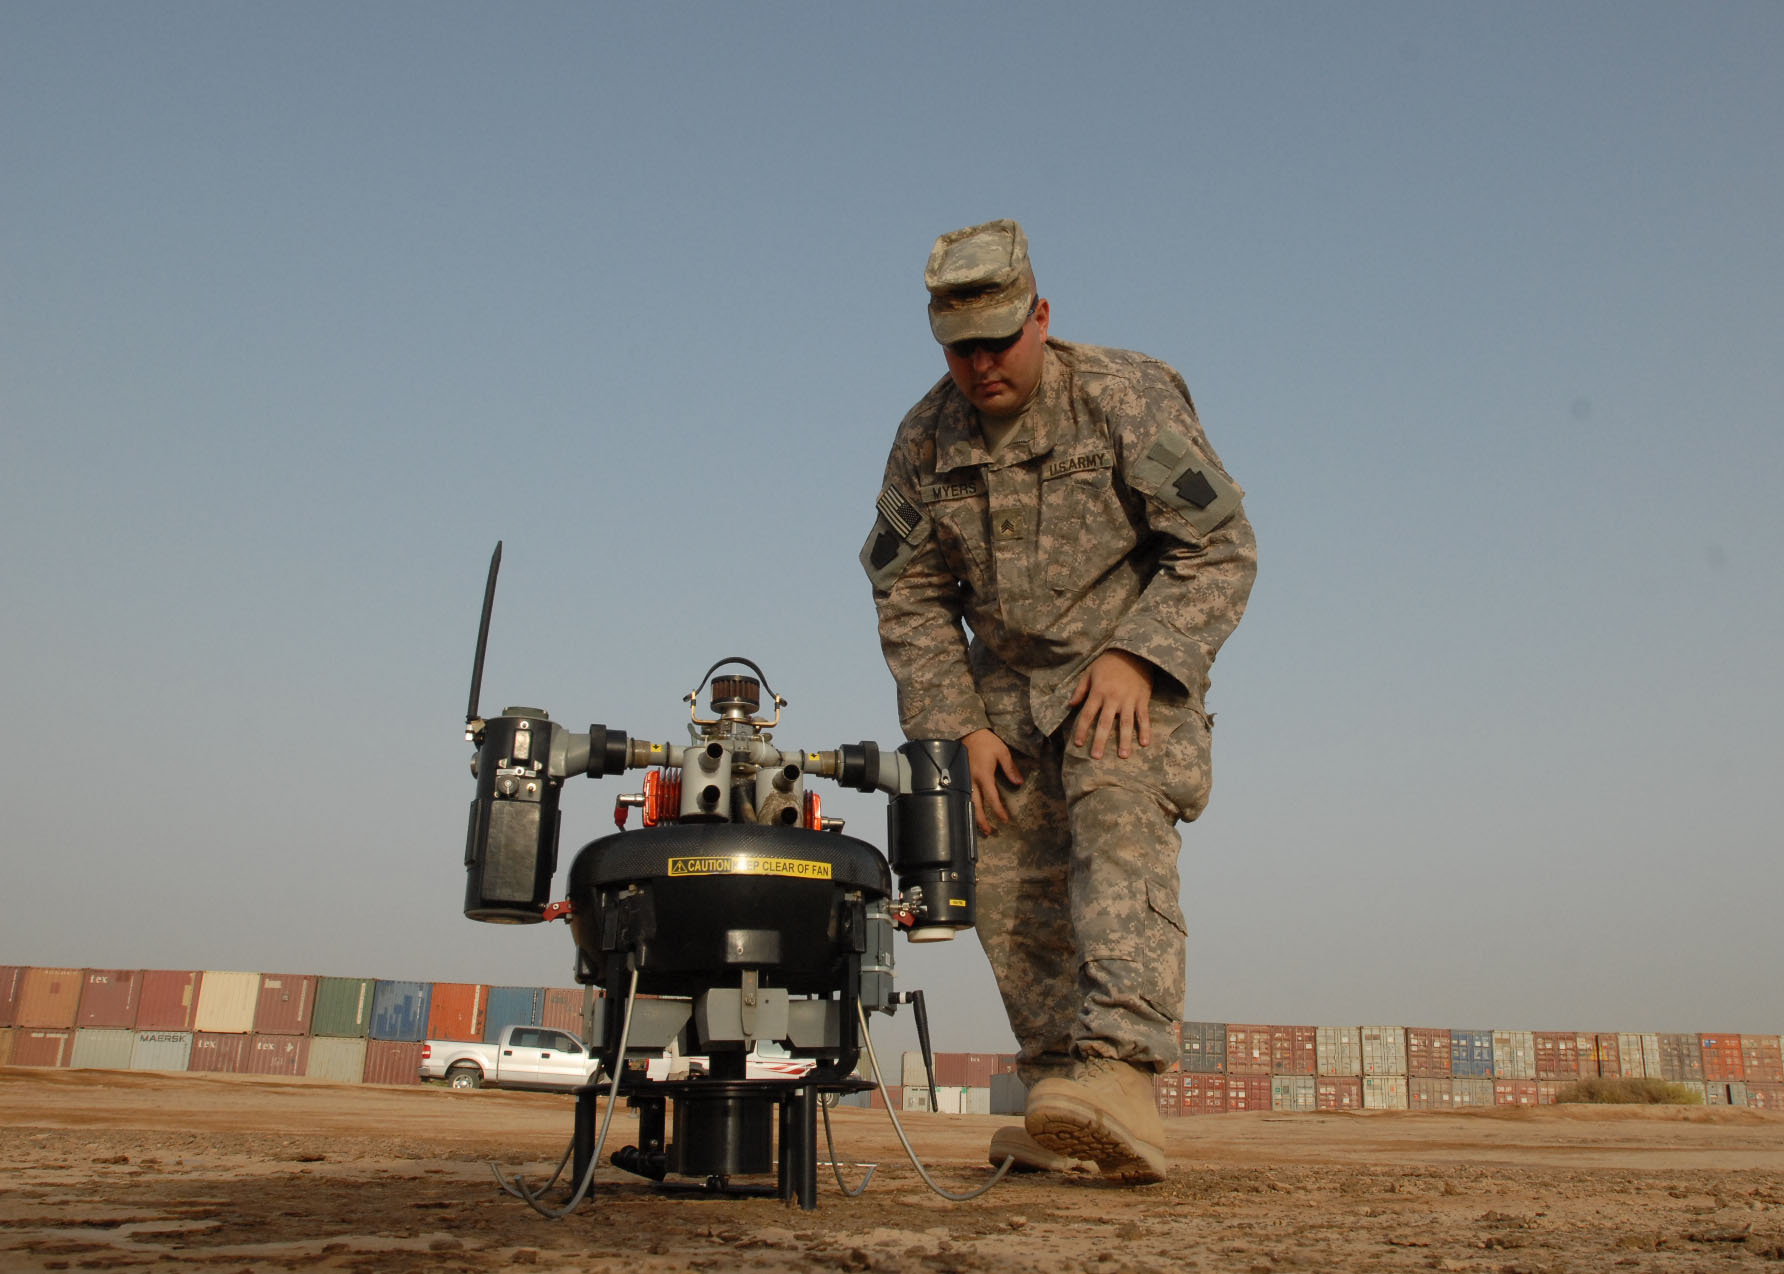
\includegraphics[width=4cm]{images/bitmap_image}
	\caption{Exemple d'image au format JPG.}
	\label{fig:une-autre-image}
\end{figure}

% Exemple figure
\textbf{\begin{figure}[htp!]
		\centering
		\setlength\figureheight{7cm}
		\setlength\figurewidth{9cm}
		% This file was created by matlab2tikz v0.2.2.
% Copyright (c) 2008--2012, Nico Schlömer <nico.schloemer@gmail.com>
% All rights reserved.
% 
% 
% 

% defining custom colors
\definecolor{mycolor1}{rgb}{0,0.75,0.75}

\begin{tikzpicture}

\begin{axis}[%
view={0}{90},
width=\figurewidth,
height=\figureheight,
scale only axis,
xmin=2, xmax=4.5,
xlabel={$\eta$},
xmajorgrids,
ymin=0.5, ymax=1,
ylabel={$d_{\text{min}}^2$},
ymajorgrids,
legend cell align=left,
legend style={align=left}]
\addplot [
color=black,
dashed,
mark=asterisk,
mark options={solid}
]
coordinates{
 (2,1)(2.1,1)(2.2,1)(2.3,1)(2.4,1)(2.5,1)(2.6,0.937749781479547)(2.7,0.890900393128398)(2.8,0.864988513955105)(2.9,0.827013168393703)(3,0.811347612650328)(3.1,0.792559278041243)(3.2,0.765840563467819)(3.3,0.749680961469385)(3.4,0.741947149227874)(3.5,0.740609493518419)(3.6,0.732128087463441)(3.7,0.717775843626632)(3.8,0.699687461812158)(3.9,0.685018622769455)(4,0.673439611642851)(4.1,0.664624248264608)(4.2,0.658255928882634)(4.3,0.641702335270489)(4.4,0.608326504614558)(4.5,0.580489221369454) 
};
\addlegendentry{$\alpha\text{ =  0\%}$};

\addplot [
color=black,
dashed,
mark=x,
mark options={solid}
]
coordinates{
 (2,1)(2.1,1)(2.2,1)(2.3,1)(2.4,0.958561324724996)(2.5,0.900812804739278)(2.6,0.859608621629443)(2.7,0.828484932127753)(2.8,0.812298837741994)(2.9,0.778916291864501)(3,0.758500630955482)(3.1,0.748375165853317)(3.2,0.745960208532468)(3.3,0.738441167434538)(3.4,0.715506361296671)(3.5,0.696927131434508)(3.6,0.682276848692725)(3.7,0.671128156410174)(3.8,0.663062783265717)(3.9,0.657680299791254)(4,0.621142740976429)(4.1,0.589786339121755)(4.2,0.564530571776849)(4.3,0.54483432747474)(4.4,0.53008799514765)(4.5,0.519641830384595) 
};
\addlegendentry{$\alpha\text{ = 10\%}$};

\addplot [
color=black,
dashed,
mark=triangle,
mark options={solid}
]
coordinates{
 (2,1)(2.1,1)(2.2,1)(2.3,0.966145915091813)(2.4,0.907589260275562)(2.5,0.862273165052718)(2.6,0.833762738286283)(2.7,0.797262289343802)(2.8,0.774689700869446)(2.9,0.763077871790574)(3,0.759584455148894)(3.1,0.735410358863577)(3.2,0.713220246811223)(3.3,0.695713299974315)(3.4,0.682371019886023)(3.5,0.672682085917092)(3.6,0.6661550402729)(3.7,0.644666127799479)(3.8,0.610083129739041)(3.9,0.582172698611821)(4,0.560333265725228)(4.1,0.543883933286703)(4.2,0.532098369213191)(4.3,0.524242326405)(4.4,0.519608701974017)(4.5,0.517545187250875) 
};
\addlegendentry{$\alpha\text{ = 20\%}$};

\addplot [
color=black,
dashed,
mark=triangle,
mark options={solid,,rotate=180}
]
coordinates{
 (2,1)(2.1,1)(2.2,0.995488894312993)(2.3,0.930050749246739)(2.4,0.882604857341179)(2.5,0.840148695151764)(2.6,0.807621264874927)(2.7,0.787889977099099)(2.8,0.777972678915356)(2.9,0.750463202108443)(3,0.726620292578349)(3.1,0.707917379352703)(3.2,0.693763185722015)(3.3,0.683575144048861)(3.4,0.676795290182409)(3.5,0.663350261880571)(3.6,0.627666127013326)(3.7,0.598755039468926)(3.8,0.575986310488554)(3.9,0.558651995817327)(4,0.546003746104731)(4.1,0.537291509323841)(4.2,0.531798375059385)(4.3,0.528867181690889)(4.4,0.527917002741411)(4.5,0.528450017604181) 
};
\addlegendentry{$\alpha\text{ = 30\%}$};

\addplot [
color=black,
dashed,
mark=o,
mark options={solid}
]
coordinates{
 (2,1)(2.1,1)(2.2,1)(2.3,1)(2.4,1)(2.5,0.995096871086856)(2.6,0.937749790013923)(2.7,0.890900391028178)(2.8,0.864988509535523)(2.9,0.827013167946275)(3,0.811347609462027)(3.1,0.79255927917077)(3.2,0.765840564829299)(3.3,0.749680963181722)(3.4,0.741947149533667)(3.5,0.740609492450166)(3.6,0.732128080624777)(3.7,0.71777584554089)(3.8,0.699687463368726)(3.9,0.681193180471954)(4,0.640212533267028)(4.1,0.617585040920557)(4.2,0.608519007405809)(4.3,0.608298095410932)(4.4,0.608326494076335)(4.5,0.580489212682311) 
};
\addlegendentry{Mazo};

\end{axis}
\end{tikzpicture}%
		\caption{Exemple de courbe TikZ.}
		\label{fig:courbe-tikz}
	\end{figure}}


% Exemple équation
\begin{align}
H_{m,n,p,q} &= \DPR{\rproto_{p,q}}{\OP{H} \tproto_{m,n}}\\
&= \iint\limits_{\SET{R}^2} S_{\OP{H}}(f,\tau) \DPR{\rproto_{p,q}}{\OP{U}_{f,\tau} \tproto_{m,n}} \ud f \ud \tau \\
&= \iint\limits_{\SET{R}^2} S_{\OP{H}}(f,\tau) \int\limits_{\R} \rproto_{p,q}^*(t) \OP{U}_{f,\tau} (\tproto_{m,n})(t) \ud t \ud f \ud \tau\\
&= \iint\limits_{\SET{R}^2} S_{\OP{H}}(f,\tau) \int\limits_{\R} \rproto^*(t-qT_0)e^{-j2 \pi pF_0t} \tproto(t-nT_0-\tau)e^{j2 \pi (mF_0(t-\tau) + ft)} \ud t \ud f \ud \tau\\
&= \iint\limits_{\SET{R}^2} S_{\OP{H}}(f,\tau) e^{-j2\pi m F_0 \tau} \int\limits_{\R} \rproto^*(t-qT_0) \tproto(t-nT_0-\tau)e^{j2 \pi ((m-p)F_0 + f)t} \ud t \ud f \ud \tau.
\end{align}